% ------------------------------------------------------------------------------
% TYPO3 Version 9.1 - What's New - Chapter "Backend User Interface" (English Version)
%
% @author	Michael Schams <schams.net>
% @license	Creative Commons BY-NC-SA 3.0
% @link		http://typo3.org/download/release-notes/whats-new/
% @language	English
% ------------------------------------------------------------------------------
% LTXE-CHAPTER-UID:		07b25346-95b1df21-a6ebe09a-49f53f41
% LTXE-CHAPTER-NAME:	Backend User Interface
% ------------------------------------------------------------------------------

\section{Backend User Interface}
\begin{frame}[fragile]
	\frametitle{Backend User Interface}

	\begin{center}\huge{Kapitel 1:}\end{center}
	\begin{center}\huge{\color{typo3darkgrey}\textbf{Backend User Interface}}\end{center}

\end{frame}

% ------------------------------------------------------------------------------
% LTXE-SLIDE-START
% LTXE-SLIDE-UID:		e0ad33fe-9f5b1a93-218b12e9-6410e8f5
% LTXE-SLIDE-TITLE:		Added New Main Module Site Management
% LTXE-SLIDE-REFERENCE:	Feature-83637-AddedNewMainModuleSiteManagement.rst
% ------------------------------------------------------------------------------

\begin{frame}[fragile]
	\frametitle{Backend User Interface}
	\framesubtitle{Site Management}

	Ein neues Hauptmodul \textbf{Site Management} wurde in den TYPO3-Core eingeführt.
	Sein Hauptzweck besteht darin, Funktionen zur Konfiguration der Seite bereit zu stellen,
	z.B. Sprachen, Domains und Routing.

	\begin{columns}[T]
		\begin{column}{.4\textwidth}
			\begin{figure}\vspace*{-0.4cm}
				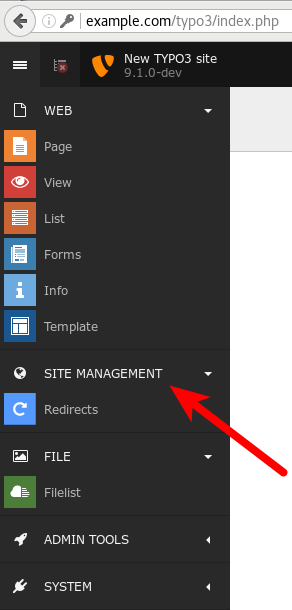
\includegraphics[width=0.45\linewidth]{BackendUserInterface/AddedNewMainModuleSiteManagement.png}
			\end{figure}
		\end{column}
		\begin{column}{.5\textwidth}
			Die neue Systemerweiterung \texttt{EXT:redirects} stellt die erste Komponente dieses
			Hauptmoduls dar (siehe nächste Seite für Details).
		\end{column}
		\begin{column}{.1\textwidth}
		\end{column}
	\end{columns}

\end{frame}

% ------------------------------------------------------------------------------
% LTXE-SLIDE-START
% LTXE-SLIDE-UID:		8bd6b85d-ed8c77e3-94a40b39-e15bb504
% LTXE-SLIDE-TITLE:		System Extension "Redirects" Has Been Added
% LTXE-SLIDE-REFERENCE:	Feature-83631-SystemExtensionRedirectsHasBeenAdded.rst
% ------------------------------------------------------------------------------

\begin{frame}[fragile]
	\frametitle{Backend User Interface}
	\framesubtitle{Weiterleitungen}

	Das neue Modul ermöglicht Integratoren und Editoren die Konfiguration von Weiterleitungen.
	Die Funktion enthält einen einfachen Hitcounter (muss aktiviert werden) und
	Weiterleitungen können unbegrenzt oder für einen bestimmten Zeitraum eingerichtet werden.

	\begin{figure}
		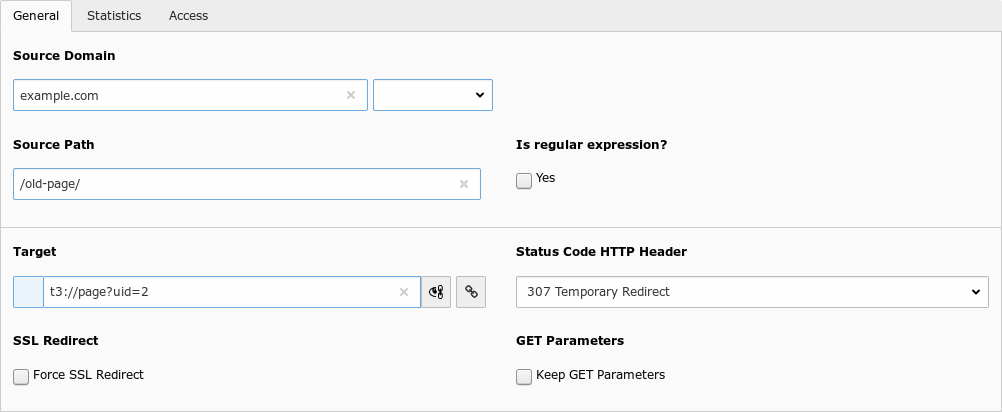
\includegraphics[width=0.8\linewidth]{BackendUserInterface/SystemExtensionRedirectsHasBeenAdded.png}
	\end{figure}

\end{frame}

% ------------------------------------------------------------------------------
% LTXE-SLIDE-START
% LTXE-SLIDE-UID:		e10a0f89-e91ecdb3-928841b6-1a84fc50
% LTXE-SLIDE-TITLE:		Show Fieldname Next To Title In Debug Mode
% LTXE-SLIDE-REFERENCE:	Feature-83461-ShowFieldnameNextToTitleInDebugMode.rst
% ------------------------------------------------------------------------------

\begin{frame}[fragile]
	\frametitle{Backend User Interface}
	\framesubtitle{Feldnamen im Debug-Modus}

	\begin{itemize}

		\item TYPO3 Integratoren und Entwickler beschäftigen sich oft mit Eingabefeldern im Backend,
			z.B. bei der Einrichtung von Berechtigungen oder während dem Schreiben von TsConfig.

		\item Anstatt in den Quellcode des Browsers zu schauen, werden Feldnamen für jedes Feld angezeigt,
			das von FormEngine generiert wird.

		\item Dies gilt nur für Benutzer mit Administratorrechten und erfordert
			dass der Denug-Modus in TYPO3 aktiviert wird.

			\smaller
				\texttt{\$GLOBALS['TYPO3\_CONF\_VARS']['BE']['debug']}
			\normalsize

	\end{itemize}

	\begin{figure}
		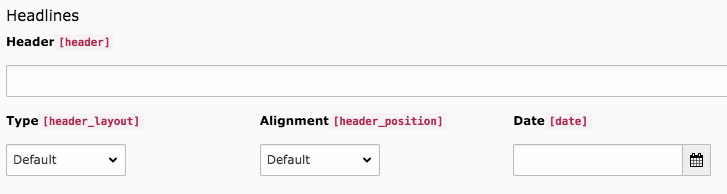
\includegraphics[width=0.60\linewidth]{BackendUserInterface/ShowFieldnameNextToTitleInDebugMode.png}
	\end{figure}

\end{frame}

% ------------------------------------------------------------------------------
